% =============================================================================
% CHAPTER 5: DESIGN PROCESS AND METHODOLOGY
% Multimodal Banglish Classroom Summarizer
% =============================================================================

\section{Introduction to the Methodology}

This chapter presents the comprehensive methodology underlying our Multimodal Banglish Classroom Summarizer, detailing the systematic approach we employed to transform raw lecture videos into structured, accurate lecture notes. The methodology addresses the fundamental challenges identified in our literature review: the absence of code-mixed ASR systems for Banglish, the complexity of multimodal information fusion without introducing hallucination, and the difficulty of evaluation under orthographic variability inherent to Romanized Bengali.

Our approach synthesizes insights from multiple research traditions. From the ASR literature, we adopt the principle of leveraging large-scale pre-trained models rather than training domain-specific systems from scratch---a practical necessity given the absence of Banglish training corpora. From the multimodal learning literature, we draw the insight that naive fusion can harm performance, leading us to develop verification-oriented approaches that treat visual information as a corrective signal rather than an unconditional bias. From the software engineering tradition, we embrace modular architecture that enables component-level evaluation and facilitates systematic experimentation.

The chapter proceeds as follows. Section 4.2 articulates our design philosophy and the constraints that shaped our architectural decisions. Section 4.3 presents the complete system architecture, detailing the audio processing pipeline, visual extraction system, cross-modal fusion mechanism, and content synthesis components. Section 4.4 describes our data collection methodology and the creation of the benchmark dataset. Section 4.5 details the preprocessing pipelines that prepare raw inputs for model processing. Section 4.6 provides implementation specifics including memory management strategies crucial for operating within hardware constraints. Finally, Section 4.7 outlines the experimental design whose results are presented in Chapter 5.

% =============================================================================
\section{Design Philosophy and Constraints}

The design of our system emerged from the intersection of ambitious research goals and practical constraints. This section articulates the philosophical principles guiding our approach and examines how real-world limitations shaped our architectural decisions.

\subsection{Guiding Principles}

Four fundamental principles informed every design decision throughout the development process, from high-level architecture to low-level implementation details.

The first principle, \textbf{leveraging pre-trained foundation models}, reflects the pragmatic reality of working with low-resource languages. Training a custom ASR system for Banglish would require hundreds of hours of transcribed code-mixed speech---data that simply does not exist. Instead, we leverage state-of-the-art pre-trained models that have learned robust acoustic and linguistic representations from massive multilingual corpora. OpenAI's Whisper \cite{Radford2023}, trained on 680,000 hours of labeled audio spanning 99 languages, provides a foundation far more capable than anything we could train from scratch. Our contribution lies not in model training but in careful prompt engineering \cite{Liu2023Prompt}, post-processing, and cross-modal integration that adapts these powerful general-purpose models to our specific domain.

The second principle, \textbf{modular pipeline architecture}, ensures that our system remains maintainable, debuggable, and extensible. Each component---audio extraction, speech recognition, visual analysis, cross-modal fusion, and content synthesis---operates as an independent module with well-defined interfaces. This modularity provides three key benefits: it enables component-level evaluation to identify performance bottlenecks; it facilitates debugging by isolating failures to specific modules; and it allows individual components to be upgraded as better models become available without requiring system-wide redesign. When a superior vision-language model emerges, we can substitute it without touching the ASR or summarization components.

The third principle, \textbf{verification over blind fusion}, emerges directly from our literature review's finding that naive multimodal fusion often harms rather than helps performance. Early experiments confirmed this concern: when we biased Whisper's output toward whiteboard keywords without verification, the system hallucinated keyword mentions where none actually occurred, degrading transcription quality. We therefore adopt a conservative approach where visual information serves primarily to verify ASR outputs and secondarily to correct high-confidence errors. This verification-oriented philosophy pervades our fusion architecture, prioritizing precision over recall to avoid introducing new errors while correcting existing ones.

The fourth principle, \textbf{practical deployment constraints}, grounds our research in real-world applicability. Academic prototypes often assume unlimited computational resources; our system must operate on accessible hardware within reasonable time constraints. We target a consumer-grade GPU with 24GB VRAM---specifically, the NVIDIA RTX 3090---which represents the upper end of hardware available to individual researchers and small institutions. This constraint drives decisions about model selection, quantization, batch processing, and memory management that might seem unnecessary in an idealized research setting but prove essential for practical deployment.

\subsection{Constraints and Their Implications}

Table~\ref{tab:constraints} summarizes the key constraints we faced and how each shaped our design decisions. These constraints are not merely limitations to be worked around; they fundamentally define the problem space and drive innovation in our approach.

\begin{table}[h]
\centering
\caption{Design Constraints and Corresponding Architectural Decisions}
\label{tab:constraints}
\begin{tabular}{|p{3.5cm}|p{4.5cm}|p{5.5cm}|}
\hline
\textbf{Constraint} & \textbf{Technical Impact} & \textbf{Design Decision} \\
\hline
No Banglish ASR training data available & Cannot train or fine-tune custom ASR models for code-mixed speech & Leverage pre-trained Whisper with domain adaptation through prompt engineering and post-processing \\
\hline
Limited GPU memory (24GB VRAM) & Cannot load multiple large models simultaneously; peak usage must stay under 24GB & Implement model registry with sequential loading; explicit memory cleanup between stages \\
\hline
Code-mixed Romanized output required & Bengali Unicode script incompatible with target format; transliteration introduces errors & Configure Whisper for English-mode output producing phonetic Romanization \\
\hline
Variable video quality across dataset & Visual extraction may fail on low-quality frames; OCR accuracy varies & Design graceful degradation allowing audio-only processing when visual extraction fails \\
\hline
No standardized Romanization for Bengali & Exact string matching fails; multiple valid spellings exist for same word & Implement fuzzy matching with configurable similarity thresholds (default 85\%) \\
\hline
Real-time processing not required & Processing time less critical than accuracy; can use larger, slower models & Prioritize model capability over inference speed; accept multi-minute processing per video \\
\hline
\end{tabular}
\end{table}

The absence of Banglish training data represents our most fundamental constraint, eliminating entire categories of potential solutions. We cannot train an end-to-end code-mixed ASR system, cannot fine-tune existing models on in-domain data, and cannot employ techniques requiring paired Banglish audio-text corpora. This constraint redirects our research from model training toward intelligent integration of existing components---a contribution that may prove more broadly applicable than a narrow domain-specific model would have been.

The GPU memory constraint of 24GB VRAM creates interesting engineering challenges. Our three primary models---Whisper large-v3-turbo (6GB), Qwen2.5-VL-7B (16GB), and Qwen2.5-7B (16GB)---cannot coexist in memory simultaneously. This necessitates a sequential processing architecture with explicit model loading and unloading between stages. While this approach increases total processing time compared to a parallel architecture, it enables us to use larger, more capable models than would otherwise be possible. The memory management system we developed, detailed in Section 4.6, ensures reliable operation without out-of-memory failures.

\subsection{Research Methodology Framework}

Our research follows an iterative experimental methodology combining systematic development with rigorous empirical evaluation. Figure~\ref{fig:methodology} illustrates the four-phase framework that structured our investigation.

% [FIGURE 5.1: Research Methodology Framework]
% Create as a horizontal flowchart with four connected phases:
%
% ┌─────────────────┐    ┌─────────────────┐    ┌─────────────────┐    ┌─────────────────┐
% │    PHASE 1      │    │    PHASE 2      │    │    PHASE 3      │    │    PHASE 4      │
% │   Requirements  │───▶│ Data Collection │───▶│ Implementation  │───▶│  Evaluation     │
% │    Analysis     │    │   & Annotation  │    │  & Integration  │    │ & Experiments   │
% └─────────────────┘    └─────────────────┘    └─────────────────┘    └─────────────────┘
%         │                      │                      │                      │
%         ▼                      ▼                      ▼                      ▼
%   ┌───────────┐          ┌───────────┐          ┌───────────┐          ┌───────────┐
%   │ Literature│          │ 9 Videos  │          │ Functional│          │ Results & │
%   │  Review   │          │ 73K chars │          │  System   │          │ Insights  │
%   │Architecture│         │Ground Truth│         │ Codebase  │          │ Chapter 6 │
%   └───────────┘          └───────────┘          └───────────┘          └───────────┘
%
% Place as Figure 5.1 after this paragraph

\textbf{Phase 1: Requirements Analysis and Architecture Design.} The first phase involved comprehensive analysis of the Banglish lecture transcription problem, surveying available tools and models, and designing a system architecture addressing identified requirements. We reviewed the ASR landscape to identify candidate models, evaluated vision-language models for whiteboard text extraction, and studied fusion architectures from the multimodal learning literature. This phase produced the modular pipeline architecture detailed in Section 4.3, along with specifications for each component.

\textbf{Phase 2: Data Collection and Ground Truth Creation.} The second phase established the empirical foundation for our research through careful data collection and annotation. We identified suitable lecture recordings from publicly available educational content, downloaded and preprocessed video files, and created manually transcribed ground truth following detailed annotation guidelines. This phase produced the benchmark dataset of nine Banglish technical lectures totaling over 73,000 characters of transcribed content, detailed in Section 4.4.

\textbf{Phase 3: Implementation and Integration.} The third phase transformed architectural designs into working code. We implemented each pipeline component, developed the model registry and memory management system, created configuration infrastructure for systematic experimentation, and integrated components into a cohesive end-to-end system. This phase also included development of the evaluation framework with term-based metrics appropriate for code-mixed content. Implementation details appear in Section 4.6.

\textbf{Phase 4: Experimentation and Evaluation.} The final phase conducted systematic experiments to evaluate system performance, compare alternative approaches, and characterize failure modes. We tested multiple configurations---baseline ASR, visual verification, conservative fusion, aggressive fusion---across all nine dataset videos. Results and analysis are presented in Chapter 5.

% =============================================================================
\section{System Architecture}

The architecture of our Multimodal Banglish Classroom Summarizer reflects a careful balance between capability and practicality. This section presents the complete system design, examining each component in detail and explaining how they interact to transform raw lecture videos into structured notes.

\subsection{High-Level Architecture Overview}

Our system follows a multimodal pipeline architecture that processes lecture videos through parallel audio and visual tracks before fusing information to produce enhanced outputs. Figure~\ref{fig:architecture} presents the complete system architecture, illustrating the flow of information from input video to final lecture notes.

% [FIGURE 5.2: High-Level System Architecture Diagram]
% Create as a professional block diagram with the following structure:
%
%                     ┌─────────────────────────┐
%                     │   INPUT: Lecture Video  │
%                     │        (.mp4)           │
%                     └───────────┬─────────────┘
%                                 │
%                     ┌───────────▼─────────────┐
%                     │    INPUT PROCESSING     │
%                     │  ┌─────────┬─────────┐  │
%                     │  │ Audio   │ Frame   │  │
%                     │  │ Extract │ Sample  │  │
%                     │  │(FFmpeg) │(OpenCV) │  │
%                     │  └────┬────┴────┬────┘  │
%                     └───────┼─────────┼───────┘
%               ┌─────────────┘         └─────────────┐
%               ▼                                     ▼
%    ┌──────────────────────┐          ┌──────────────────────┐
%    │    AUDIO TRACK       │          │    VISUAL TRACK      │
%    │  ┌────────────────┐  │          │  ┌────────────────┐  │
%    │  │    Whisper     │  │          │  │   Qwen2.5-VL   │  │
%    │  │ large-v3-turbo │  │          │  │  7B-Instruct   │  │
%    │  └───────┬────────┘  │          │  └───────┬────────┘  │
%    │          ▼           │          │          ▼           │
%    │  ┌────────────────┐  │          │  ┌────────────────┐  │
%    │  │  Transcript    │  │          │  │   Keywords &   │  │
%    │  │   Cleaning     │  │          │  │  Aggregation   │  │
%    │  └───────┬────────┘  │          │  └───────┬────────┘  │
%    └──────────┼───────────┘          └──────────┼───────────┘
%               └─────────────┐   ┌───────────────┘
%                             ▼   ▼
%                  ┌──────────────────────────┐
%                  │   CROSS-MODAL FUSION     │
%                  │ • Keyword Verification   │
%                  │ • Confidence Weighting   │
%                  │ • Anti-Hallucination     │
%                  └────────────┬─────────────┘
%                               ▼
%                  ┌──────────────────────────┐
%                  │   CONTENT SYNTHESIS      │
%                  │     Qwen2.5-7B-Instruct  │
%                  │   Lecture Note Generation│
%                  └────────────┬─────────────┘
%                               ▼
%                  ┌──────────────────────────┐
%                  │  OUTPUT: Structured      │
%                  │     Lecture Notes        │
%                  └──────────────────────────┘
%
% Use Draw.io or TikZ. Place as Figure 5.2.

The pipeline consists of five major stages, each designed as an independent module with well-defined interfaces. The \textbf{Input Processing} stage decomposes the video into audio and visual streams using FFmpeg for audio extraction and OpenCV for frame sampling. The \textbf{Audio Track Processing} stage employs Whisper for speech recognition followed by transcript cleaning to remove hallucinations and normalize format. The \textbf{Visual Track Processing} stage uses Qwen2.5-VL to extract whiteboard content and technical keywords from sampled frames, aggregating results across the video timeline. The \textbf{Cross-Modal Fusion} stage combines information from both tracks, using visual keywords to verify and selectively correct ASR outputs while implementing safeguards against hallucination. Finally, the \textbf{Content Synthesis} stage employs Qwen2.5 to generate structured lecture notes from the fused transcript and visual context.

This modular design enables systematic experimentation: we can evaluate each component independently, swap alternative implementations, and isolate the source of errors when they occur.

\subsection{Component Specifications}

Table~\ref{tab:components} provides a comprehensive overview of all system components, including the specific models and tools employed, their primary functions, and their computational requirements. The VRAM column indicates GPU memory consumption, which drives our sequential loading strategy discussed in Section 4.6.

\begin{table}[h]
\centering
\caption{System Component Specifications and Resource Requirements}
\label{tab:components}
\begin{tabular}{|l|l|p{5cm}|c|}
\hline
\textbf{Component} & \textbf{Model/Tool} & \textbf{Function} & \textbf{VRAM} \\
\hline
Audio Extraction & FFmpeg 6.0 & Extracts audio track from video, converts to 16kHz mono WAV & CPU only \\
\hline
Frame Sampling & OpenCV 4.8.0 & Samples frames at configurable intervals, saves as JPEG & CPU only \\
\hline
Speech Recognition & Whisper large-v3-turbo & Transcribes speech to text with timestamps; 809M parameters & 6 GB \\
\hline
Visual Analysis & Qwen2.5-VL-7B-Instruct & Extracts whiteboard text and technical keywords from frames & 16 GB \\
\hline
Content Synthesis & Qwen2.5-7B-Instruct & Generates structured lecture notes from transcript and keywords & 16 GB \\
\hline
Text Processing & Python 3.10 + RapidFuzz & Cleaning, fuzzy matching, fusion logic, evaluation metrics & CPU only \\
\hline
\end{tabular}
\end{table}

The table reveals why sequential model loading is necessary: Whisper, Qwen2.5-VL, and Qwen2.5 together would require 38GB of VRAM, exceeding our 24GB constraint. By loading only one large model at a time and explicitly releasing memory between stages, we accommodate all three models within available resources.

\subsection{Audio Processing Pipeline}

The audio processing pipeline transforms raw video audio into cleaned transcriptions suitable for fusion and summarization. This section details each stage of audio processing, from extraction through cleaning.

\subsubsection{Audio Extraction and Preparation}

Audio extraction represents the first computational step in our pipeline. We employ FFmpeg, the industry-standard multimedia framework, to extract the audio track from input videos and convert it to Whisper's expected format: 16kHz mono audio encoded as 16-bit PCM in an uncompressed WAV container. This specification ensures compatibility with Whisper's mel spectrogram computation while avoiding codec artifacts that could degrade transcription quality.

The conversion process is implemented as a single FFmpeg command that handles resampling, channel mixing, and format conversion atomically:

\begin{verbatim}
ffmpeg -i input.mp4 -ar 16000 -ac 1 -c:a pcm_s16le output.wav
\end{verbatim}

This command reads the input video, extracts the audio track, resamples to 16kHz, downmixes to mono, and encodes as 16-bit PCM WAV. The process typically completes in under one second for a ten-minute video, making it negligible in the overall processing time.

\subsubsection{Speech Recognition with Whisper}

The heart of our audio processing pipeline is OpenAI's Whisper large-v3-turbo model \cite{Radford2023}, a state-of-the-art multilingual ASR system trained on approximately 680,000 hours of labeled audio. We selected this variant for its balance of accuracy and computational efficiency: it achieves performance comparable to the full large-v3 model while requiring significantly less inference time. The model architecture follows the encoder-decoder Transformer paradigm \cite{Vaswani2017}, processing log-Mel spectrograms through attention mechanisms that have proven highly effective for sequence-to-sequence tasks \cite{Sutskever2014}.

Table~\ref{tab:whisper_config} details our Whisper configuration, with each parameter carefully chosen for the Banglish lecture domain.

\begin{table}[h]
\centering
\caption{Whisper Model Configuration for Banglish Lecture Transcription}
\label{tab:whisper_config}
\begin{tabular}{|l|l|p{6.5cm}|}
\hline
\textbf{Parameter} & \textbf{Value} & \textbf{Rationale} \\
\hline
Model Variant & large-v3-turbo & Best accuracy-speed tradeoff; 809M parameters \\
\hline
Language & English & Outputs Romanized text; captures technical terms accurately \\
\hline
Task & Transcribe & Transcription rather than translation preserves original speech \\
\hline
Beam Size & 5 & Sufficient for quality without excessive computation \\
\hline
Temperature & 0.0 & Deterministic output ensures reproducibility \\
\hline
Condition on Previous & True & Maintains context across 30-second segments \\
\hline
VAD Filter & Enabled & Removes silence; reduces hallucination in quiet segments \\
\hline
Word Timestamps & Enabled & Provides temporal alignment for fusion \\
\hline
\end{tabular}
\end{table}

% [FIGURE 5.3: Whisper ASR Processing Flow]
% Create as a vertical flowchart showing:
%
%    ┌─────────────────────────────┐
%    │  Input: 16kHz Mono Audio   │
%    └─────────────┬───────────────┘
%                  │
%    ┌─────────────▼───────────────┐
%    │   Log-Mel Spectrogram      │
%    │   80 bins × 30s chunks     │
%    └─────────────┬───────────────┘
%                  │
%    ┌─────────────▼───────────────┐
%    │   Transformer Encoder      │
%    │      (32 layers)           │
%    │   Acoustic Representation  │
%    └─────────────┬───────────────┘
%                  │
%    ┌─────────────▼───────────────┐
%    │   Transformer Decoder      │
%    │      (32 layers)           │
%    │  + Language/Task Tokens    │
%    └─────────────┬───────────────┘
%                  │
%    ┌─────────────▼───────────────┐
%    │  Token-by-Token Generation │
%    │  with Beam Search (k=5)    │
%    └─────────────┬───────────────┘
%                  │
%    ┌─────────────▼───────────────┐
%    │  Output: Raw Transcript    │
%    │    + Word Timestamps       │
%    └─────────────────────────────┘
%
% Place as Figure 5.3.

The decision to configure Whisper for English output, despite processing Banglish content, merits detailed explanation. When configured for Bengali, Whisper outputs text in Bengali Unicode script (বাংলা), which is incompatible with our Romanized ground truth and would require lossy transliteration for evaluation. In English mode, Whisper produces Romanized approximations of Bengali words---``korbo'' becomes ``curb oh'' or similar phonetic renderings---which, while imperfect, are directly comparable to our Romanized ground truth. More importantly, English mode accurately captures technical terms (``variable,'' ``function,'' ``polymorphism'') that constitute our primary evaluation focus.

Figure~\ref{fig:whisper_flow} illustrates the internal processing flow within Whisper. Audio is first converted to a log-Mel spectrogram with 80 frequency bins \cite{Davis1980}, then processed in 30-second chunks by a 32-layer Transformer encoder to produce acoustic representations. The 32-layer Transformer decoder, conditioned on task and language tokens, generates text tokens autoregressively using beam search with beam width 5. Word-level timestamps are extracted from attention patterns \cite{Luong2015}, providing temporal alignment information used in cross-modal fusion.

\subsubsection{Transcript Cleaning and Hallucination Removal}

Raw Whisper output frequently contains artifacts that degrade downstream processing quality. Our cleaning pipeline addresses three categories of issues: repetition hallucinations, stock phrase insertions, and format inconsistencies.

\textbf{Repetition Hallucination} represents the most common failure mode, where Whisper produces looping patterns like ``the the the the the'' or ``and and and and.'' These typically occur during silence, background noise, or unclear speech segments---a phenomenon well-documented in neural text generation \cite{Holtzman2020, Ji2023}. We detect repetitions using n-gram analysis: any word or phrase appearing more than five consecutive times triggers removal of excess repetitions, preserving at most two instances.

\textbf{Stock Phrase Hallucination} occurs when Whisper inserts phrases common in its training data but absent from the actual audio. Phrases like ``thank you for watching,'' ``please subscribe,'' and ``like and share'' appear frequently in YouTube training data and occasionally hallucinate into lecture transcripts. We maintain a blocklist of such phrases and remove them when detected.

\textbf{Format Normalization} ensures consistency across transcripts for reliable evaluation. The cleaning pipeline applies the following rules sequentially: (1) \textit{repetition removal}, reducing sequences of more than five consecutive identical words/phrases to at most two instances; (2) \textit{stock phrase filtering}, removing YouTube-specific phrases like ``thank you for watching'' and ``please subscribe''; (3) \textit{punctuation cleanup}, normalizing excessive punctuation to single instances; (4) \textit{case normalization}, converting all text to lowercase; (5) \textit{whitespace collapse}, replacing multiple spaces, tabs, and newlines with single spaces; and (6) \textit{Unicode normalization}, converting all text to NFC form for consistent character representation.

\subsection{Visual Processing Pipeline}

While the audio track captures the instructor's spoken words, the visual track provides complementary information through whiteboard content, code demonstrations, and written keywords. The visual processing pipeline extracts this information and prepares it for fusion with the audio transcript.

\subsubsection{Frame Sampling Strategy}

Classroom lecture videos present a unique visual challenge: content changes slowly as instructors write on whiteboards, with long periods where frames are nearly identical. Processing every frame would waste computation on redundant content; sampling too sparsely risks missing important material. We conducted empirical analysis to determine optimal sampling intervals, with results summarized in Table~\ref{tab:sampling}.

\begin{table}[h]
\centering
\caption{Frame Sampling Interval Analysis: Coverage vs. Efficiency Tradeoff}
\label{tab:sampling}
\begin{tabular}{|c|c|c|c|c|c|}
\hline
\textbf{Interval} & \textbf{Frames/Min} & \textbf{VLM Calls} & \textbf{Processing} & \textbf{Keyword} & \textbf{Frame} \\
\textbf{(seconds)} & & \textbf{per 10min} & \textbf{Time} & \textbf{Coverage} & \textbf{Redundancy} \\
\hline
10 & 6 & 60 & 12 min & 98\% & 72\% \\
\hline
20 & 3 & 30 & 6 min & 95\% & 45\% \\
\hline
30 & 2 & 20 & 4 min & 89\% & 28\% \\
\hline
\end{tabular}
\end{table}

The analysis reveals a clear tradeoff: shorter intervals capture more keywords but with diminishing returns as redundancy increases. At 10-second intervals, 72\% of extracted content duplicates information from adjacent frames; reducing to 20-second intervals sacrifices only 3\% of keyword coverage while halving processing time and significantly reducing redundancy. We selected 20-second intervals as the default, though the system supports configurable intervals for different use cases.

% [FIGURE 5.4: Frame Sampling Timeline Visualization]
% Create as a horizontal timeline diagram:
%
%    Video Timeline (10-minute lecture)
%    ├────┬────┬────┬────┬────┬────┬────┬────┬────┬────┤
%    0   1    2    3    4    5    6    7    8    9   10 min
%    
%    20-second Sampling Points:
%    ▼    ▼    ▼    ▼    ▼    ▼    ▼    ▼    ▼    ▼    ▼ ...
%    │    │    │    │    │    │    │    │    │    │    │
%    ┌────┴────┬────┴────┬────┴────┬────┴────┬────┴────┐
%    │ Frame 1 │ Frame 2 │ Frame 3 │ Frame 4 │ Frame 5 │ ...
%    │ 0:00    │ 0:20    │ 0:40    │ 1:00    │ 1:20    │
%    │         │         │         │         │         │
%    │[python] │[python] │[variable│[variable│[print]  │
%    │[intro]  │[variable│ =value] │ input]  │[output] │
%    └─────────┴─────────┴─────────┴─────────┴─────────┘
%
%    Total: 30 frames for 10-minute video at 20s intervals
%
% Place as Figure 5.4.

Figure~\ref{fig:frame_sampling} illustrates the sampling strategy applied to a 10-minute lecture. Frames are extracted at 0:00, 0:20, 0:40, and so forth, resulting in 30 frames for a 10-minute video. Each frame is timestamped, enabling temporal alignment with the audio transcript during fusion.

\subsubsection{Visual Content Extraction with Qwen2.5-VL}

For visual content extraction, we employ Qwen2.5-VL-7B-Instruct \cite{Wang2024Qwen2VL}, a state-of-the-art vision-language model with strong capabilities in document understanding, OCR, and scene description. The model builds upon advances in vision-language pre-training \cite{Radford2021, Li2023BLIP2} and document understanding architectures \cite{Xu2020LayoutLM}. The model processes each sampled frame to extract multiple categories of information, as detailed in Table~\ref{tab:visual_extraction}.

\begin{table}[h]
\centering
\caption{Visual Content Extraction Categories and Examples}
\label{tab:visual_extraction}
\begin{tabular}{|l|p{5cm}|p{5.5cm}|}
\hline
\textbf{Category} & \textbf{Description} & \textbf{Example Extractions} \\
\hline
Whiteboard Text & All visible handwritten or printed text on whiteboard/screen & ``Variables store data values'', ``x = 5'' \\
\hline
Technical Keywords & Domain-specific terms and concepts & ``variable'', ``integer'', ``string'', ``print'' \\
\hline
Code Snippets & Programming code visible in frame & \texttt{name = input("Enter name:")} \\
\hline
Diagram Descriptions & Textual descriptions of visual diagrams & ``Flowchart showing if-else branching'' \\
\hline
Structural Elements & Headings, lists, hierarchical organization & ``Section: Data Types'', ``1. int 2. float 3. str'' \\
\hline
\end{tabular}
\end{table}

The extraction process uses a carefully engineered prompt that instructs the model to provide structured output in JSON format:

\begin{quote}
\textit{``You are analyzing a frame from an educational lecture video. The frame shows a whiteboard or screen with instructional content. Your task is to extract ALL visible text and identify key educational elements.}

\textit{Please provide your response in JSON format with the following fields:}
\begin{itemize}
    \item \textit{whiteboard\_text: Complete transcription of all visible text}
    \item \textit{keywords: List of technical terms and important concepts}
    \item \textit{code: Any programming code visible (preserve formatting)}
    \item \textit{diagrams: Descriptions of any diagrams or visual aids}
    \item \textit{structure: Organizational elements (headings, lists)}
\end{itemize}
\textit{Be thorough---extract everything visible, even if partially obscured.''}
\end{quote}

This prompt design ensures consistent, structured output across frames while encouraging comprehensive extraction. The JSON format enables programmatic parsing and aggregation of results.

\subsubsection{Keyword Aggregation and Confidence Scoring}

Content extracted from multiple frames is aggregated to produce a unified visual context. The aggregation process addresses several challenges: the same keyword appears in multiple consecutive frames as it remains on the whiteboard; OCR errors may produce slightly different extractions of the same text; and historical content may persist visually after the instructor has moved on to new topics.

% [FIGURE 5.5: Visual Keyword Aggregation Process]
% Create as a diagram showing:
%
%    FRAME-LEVEL EXTRACTIONS
%    ┌─────────────┐  ┌─────────────┐  ┌─────────────┐  ┌─────────────┐
%    │  Frame 1    │  │  Frame 2    │  │  Frame 3    │  │  Frame 4    │
%    │  (0:00)     │  │  (0:20)     │  │  (0:40)     │  │  (1:00)     │
%    ├─────────────┤  ├─────────────┤  ├─────────────┤  ├─────────────┤
%    │ • variable  │  │ • variable  │  │ • variable  │  │ • input     │
%    │ • Python    │  │ • integer   │  │ • integer   │  │ • integer   │
%    │             │  │ • string    │  │ • string    │  │ • string    │
%    │             │  │             │  │ • input     │  │ • print     │
%    └──────┬──────┘  └──────┬──────┘  └──────┬──────┘  └──────┬──────┘
%           │                │                │                │
%           └────────────────┴────────────────┴────────────────┘
%                                    │
%                                    ▼
%                         ┌─────────────────────┐
%                         │    AGGREGATION      │
%                         │  • Deduplication    │
%                         │  • Confidence Score │
%                         │  • Noise Filtering  │
%                         └──────────┬──────────┘
%                                    │
%                                    ▼
%                    ┌───────────────────────────────┐
%                    │  UNIFIED KEYWORD SET          │
%                    ├───────────────────────────────┤
%                    │  variable  : conf=4, t=0:00   │
%                    │  integer   : conf=3, t=0:20   │
%                    │  string    : conf=3, t=0:20   │
%                    │  input     : conf=2, t=0:40   │
%                    │  Python    : conf=1, t=0:00   │
%                    │  print     : conf=1, t=1:00   │
%                    └───────────────────────────────┘
%
% Place as Figure 5.5.

Our aggregation algorithm proceeds as follows. First, we collect all keywords extracted from all frames. Second, we apply fuzzy deduplication using string similarity: keywords with similarity above 90\% are considered identical, with the most common spelling retained. Third, we compute a confidence score for each unique keyword based on the number of frames in which it appeared---a keyword visible in more frames is more likely to be important and correctly extracted. Fourth, we record the timestamp of first appearance for each keyword, enabling temporal alignment during fusion. Finally, we apply noise filtering to remove low-confidence extractions: single-character strings, common stop words, and keywords appearing in only one frame with low OCR confidence are discarded.

Table~\ref{tab:aggregation_example} illustrates this process with a concrete example from our dataset.

\begin{table}[h]
\centering
\caption{Keyword Aggregation Example from BanglaASR2 (Python Input Functions)}
\label{tab:aggregation_example}
\begin{tabular}{|l|c|c|l|}
\hline
\textbf{Keyword} & \textbf{Frame Count} & \textbf{Confidence} & \textbf{First Seen} \\
\hline
input & 8 & High & 0:45 \\
\hline
variable & 6 & High & 0:20 \\
\hline
print & 5 & High & 1:30 \\
\hline
string & 4 & Medium & 0:40 \\
\hline
int & 3 & Medium & 2:15 \\
\hline
float & 2 & Medium & 3:00 \\
\hline
Python & 1 & Low & 0:00 \\
\hline
\end{tabular}
\end{table}

\subsection{Cross-Modal Fusion Architecture}

The fusion stage represents the intellectual core of our multimodal approach, combining information from audio and visual tracks to produce transcriptions superior to either modality alone. Our design philosophy prioritizes verification over blind integration: visual information serves primarily to verify ASR outputs and secondarily to correct high-confidence errors.

\subsubsection{The Fusion Challenge}

Naive approaches to multimodal fusion can degrade rather than improve performance. Our early experiments with aggressive visual biasing---forcing Whisper to prefer visually-extracted keywords---resulted in significant hallucination: the system would insert keywords into the transcript where they were never spoken, simply because they appeared on the whiteboard. A term written at minute 2 might be hallucinated into the transcript at minutes 5, 8, and 12, corrupting otherwise accurate transcription.

This observation motivated our verification-oriented approach. Rather than using visual keywords to bias ASR during recognition, we use them to verify and selectively correct ASR outputs post-hoc. This conservative strategy sacrifices some potential improvement for safety against hallucination.

\subsubsection{Verification and Correction Process}

The fusion process operates in three stages: verification, correction, and anti-hallucination filtering. Figure~\ref{fig:fusion_flow} illustrates the complete fusion workflow.

% [FIGURE 5.6: Cross-Modal Fusion Flowchart]
% Create as a detailed flowchart:
%
%    ┌─────────────────┐     ┌─────────────────┐
%    │  ASR Transcript │     │ Visual Keywords │
%    │  with Timestamps│     │ with Timestamps │
%    └────────┬────────┘     └────────┬────────┘
%             │                       │
%             └───────────┬───────────┘
%                         │
%                         ▼
%              ┌─────────────────────┐
%              │  STAGE 1: VERIFY    │
%              │  For each ASR term: │
%              │  Find matching      │
%              │  visual keyword     │
%              └──────────┬──────────┘
%                         │
%            ┌────────────┼────────────┐
%            ▼            ▼            ▼
%     ┌──────────┐ ┌──────────┐ ┌──────────┐
%     │sim > 85% │ │60-84% sim│ │sim < 60% │
%     │ VERIFIED │ │ CANDIDATE│ │NO MATCH  │
%     └────┬─────┘ └────┬─────┘ └────┬─────┘
%          │            │            │
%          ▼            ▼            ▼
%     ┌──────────┐ ┌──────────┐ ┌──────────┐
%     │Keep ASR  │ │Check vis │ │Keep ASR  │
%     │as-is     │ │confidence│ │as-is     │
%     └──────────┘ └────┬─────┘ └──────────┘
%                       │
%            ┌──────────┼──────────┐
%            ▼          ▼          ▼
%     ┌──────────┐ ┌──────────┐ ┌──────────┐
%     │High conf │ │Med conf  │ │Low conf  │
%     │SUBSTITUTE│ │FLAG      │ │KEEP ASR  │
%     └──────────┘ └──────────┘ └──────────┘
%                       │
%                       ▼
%              ┌─────────────────────┐
%              │ STAGE 3: ANTI-HALL  │
%              │ Check frequency,    │
%              │ temporal locality   │
%              └──────────┬──────────┘
%                         │
%                         ▼
%              ┌─────────────────────┐
%              │   FUSED TRANSCRIPT  │
%              └─────────────────────┘
%
% Place as Figure 5.6.

\textbf{Stage 1: Verification.} For each term in the ASR transcript, we search for matching visual keywords using fuzzy string matching \cite{Cohen2003}. The similarity score is computed as the normalized Levenshtein distance ratio \cite{Levenshtein1966}:

\begin{equation}
\text{similarity}(s_1, s_2) = 1 - \frac{\text{levenshtein}(s_1, s_2)}{\max(|s_1|, |s_2|)}
\end{equation}

Terms with similarity above 85\% are marked as \textit{verified}---the ASR output matches visual evidence and is retained as-is. Terms with similarity between 60-84\% are marked as \textit{correction candidates}---the ASR output may be a garbled version of the visual keyword. Terms with similarity below 60\% have \textit{no match}---no visual evidence supports or contradicts the ASR output.

\textbf{Stage 2: Selective Correction.} For correction candidates, we apply a conservative correction strategy based on visual confidence. Table~\ref{tab:correction_strategy} summarizes the decision logic.

\begin{table}[h]
\centering
\caption{Correction Strategy Based on Match Quality and Visual Confidence}
\label{tab:correction_strategy}
\begin{tabular}{|c|c|l|}
\hline
\textbf{Similarity} & \textbf{Visual Confidence} & \textbf{Action} \\
\hline
$\geq$ 85\% & Any & Keep ASR (verified) \\
\hline
60-84\% & High ($\geq$3 frames) & Substitute visual keyword \\
\hline
60-84\% & Medium (2 frames) & Keep ASR, flag for review \\
\hline
60-84\% & Low (1 frame) & Keep ASR \\
\hline
$<$ 60\% & Any & Keep ASR (no match) \\
\hline
\end{tabular}
\end{table}

This conservative approach ensures corrections occur only when visual evidence is strong. A keyword seen in three or more frames is almost certainly correct; a keyword seen in only one frame may be an OCR error.

\textbf{Stage 3: Anti-Hallucination Filtering.} Even with conservative correction, visual keywords could theoretically be inserted where they were never spoken. We implement additional safeguards:

\begin{enumerate}
    \item \textbf{Temporal Locality:} Visual keywords can only influence ASR terms within $\pm$60 seconds of the keyword's first appearance timestamp. A term written at minute 5 cannot trigger corrections at minute 1 or minute 10.
    
    \item \textbf{Frequency Limiting:} Each visual keyword can trigger at most 3 corrections per lecture. This prevents a single prominent whiteboard term from being inserted throughout the transcript.
    
    \item \textbf{Context Compatibility:} Before substitution, we verify that surrounding context is semantically compatible. A keyword like ``polymorphism'' should not be inserted into a segment discussing basic arithmetic.
\end{enumerate}

% [FIGURE 5.6: Keyword Verification Flow]
% Already covered in Figure 5.6 above - remove this duplicate

\subsection{Content Synthesis Pipeline}

The final pipeline stage transforms the fused transcript and visual context into structured, student-friendly lecture notes. This synthesis task requires not merely summarization but intelligent reorganization of spoken content into a coherent written format.

\subsubsection{Summarization Model Selection and Configuration}

We employ Qwen2.5-7B-Instruct \cite{Bai2023Qwen} for content synthesis, selected for its strong instruction-following capabilities and generous context window. This model exemplifies the trend toward instruction-tuned language models \cite{Ouyang2022} that can follow complex, multi-step directives. Table~\ref{tab:summarization_config} details the model configuration.

\begin{table}[h]
\centering
\caption{Content Synthesis Model Configuration}
\label{tab:summarization_config}
\begin{tabular}{|l|l|p{6cm}|}
\hline
\textbf{Parameter} & \textbf{Value} & \textbf{Rationale} \\
\hline
Model & Qwen2.5-7B-Instruct & Strong instruction following; multilingual capability \\
\hline
Parameters & 7.6 billion & Balance of capability and resource requirements \\
\hline
Quantization & 4-bit (GPTQ) & Reduces VRAM to $\sim$6GB while maintaining quality \\
\hline
Context Window & 32,768 tokens & Accommodates full transcripts of long lectures \\
\hline
Temperature & 0.3 & Slight creativity for natural phrasing; mostly deterministic \\
\hline
Top-p & 0.9 & Nucleus sampling for diversity within constraints \\
\hline
Max Output & 4,096 tokens & Sufficient for comprehensive lecture notes \\
\hline
\end{tabular}
\end{table}

The use of 4-bit quantization merits explanation. Full-precision Qwen2.5-7B requires approximately 16GB of VRAM, leaving insufficient room for processing overhead on our 24GB GPU. Quantization to 4-bit precision reduces memory requirements to approximately 6GB with minimal quality degradation---studies have shown that 4-bit quantized models retain 95-99\% of full-precision performance on text generation tasks.

\subsubsection{Prompt Engineering for Educational Content}

The quality of generated lecture notes depends critically on prompt design. Our prompt provides explicit instructions for structure, style, and content handling:

\begin{quote}
\textit{``You are an expert educational content creator specializing in technical subjects. Your task is to transform a lecture transcript into comprehensive, well-structured study notes that will help students learn effectively.}

\textit{LECTURE TRANSCRIPT:}
\textit{[Cleaned and fused transcript]}

\textit{WHITEBOARD KEYWORDS (important terms written by instructor):}
\textit{[Aggregated visual keywords with confidence scores]}

\textit{Please create lecture notes following these guidelines:}
\begin{enumerate}
    \item \textit{Begin with a clear title reflecting the lecture topic}
    \item \textit{Provide a 2-3 sentence overview summarizing the main points}
    \item \textit{Organize content under logical headings and subheadings}
    \item \textit{Define technical terms when first introduced}
    \item \textit{Include code examples with proper formatting if discussed}
    \item \textit{Use the whiteboard keywords as anchors for important concepts}
    \item \textit{Correct obvious transcription errors using context}
    \item \textit{Conclude with a summary of key takeaways}
\end{enumerate}
\textit{The output should be in Markdown format suitable for student study.''}
\end{quote}

This prompt structure guides the model to produce consistently formatted, educationally useful output while leveraging both transcript content and visual keyword context.

\subsubsection{Output Structure and Quality}

Generated lecture notes follow a consistent structure designed for student utility. Table~\ref{tab:note_structure} describes each section.

\begin{table}[h]
\centering
\caption{Generated Lecture Note Structure}
\label{tab:note_structure}
\begin{tabular}{|l|p{5cm}|p{5.5cm}|}
\hline
\textbf{Section} & \textbf{Content} & \textbf{Purpose} \\
\hline
Title & Lecture topic derived from content & Quick identification of subject matter \\
\hline
Overview & 2-3 sentence summary & Provides context before detailed reading \\
\hline
Key Concepts & Bulleted list of main topics & Serves as study checklist \\
\hline
Detailed Notes & Organized content with headings & Primary learning material \\
\hline
Code Examples & Formatted code blocks & Demonstrates practical application \\
\hline
Summary & Key takeaways and review points & Facilitates review and retention \\
\hline
\end{tabular}
\end{table}

% =============================================================================
\section{Data Collection and Benchmark Creation}

The creation of a benchmark dataset represents a fundamental contribution of this research, providing the first ground-truth annotated corpus for Banglish technical lecture transcription. This section details our data collection methodology, annotation procedures, and quality assurance processes.

\subsection{Dataset Requirements Analysis}

Before collecting data, we established requirements that the benchmark dataset must satisfy to enable meaningful research. These requirements emerged from our analysis of the research gap and practical deployment considerations.

\textbf{Requirement 1: Authentic Code-Mixing.} The dataset must contain natural Banglish as actually used in Bangladeshi technical education, not artificially constructed code-mixed content. This authenticity is essential for evaluating systems intended for real-world deployment.

\textbf{Requirement 2: Technical Domain Coverage.} The dataset must span multiple technical domains to assess generalization across vocabulary and subject matter. We targeted at least three distinct domains with different technical terminology.

\textbf{Requirement 3: Visual Content.} Videos must feature whiteboard instruction with visible written content, enabling evaluation of our multimodal approach. Pure lecture-style videos without visual aids were excluded.

\textbf{Requirement 4: Realistic Acoustic Conditions.} Recordings must reflect real classroom environments with typical noise, reverberation, and recording quality---not studio-produced content that would overestimate real-world performance.

\textbf{Requirement 5: Sufficient Scale.} The dataset must be large enough for meaningful quantitative evaluation while remaining feasible for manual ground truth creation. We targeted approximately 70,000+ characters of transcribed content.

\subsection{Source Selection and Collection}

We identified YouTube as the primary source for lecture recordings, offering abundant Bangladeshi educational content that is legally accessible for research purposes. Our selection process applied the following criteria systematically.

Videos were included if they featured: (1) an instructor speaking in Banglish with natural code-mixing; (2) technical subject matter in computer science or engineering; (3) visible whiteboard or screen content; (4) intelligible speech quality; and (5) duration between 5-30 minutes. Videos were excluded if they featured: (1) predominantly one language without code-mixing; (2) purely verbal instruction without visual aids; (3) severely degraded audio quality; or (4) copyrighted content requiring special permissions.

\subsection{Final Dataset Composition}

The final benchmark dataset comprises nine lecture recordings totaling over 73,000 characters of ground truth transcription. Table~\ref{tab:dataset_full} provides comprehensive details for each video.

\begin{table}[h]
\centering
\caption{Complete Benchmark Dataset Specification}
\label{tab:dataset_full}
\begin{tabular}{|l|p{4.5cm}|c|c|c|}
\hline
\textbf{Video ID} & \textbf{Topic} & \textbf{Domain} & \textbf{GT Chars} & \textbf{Keywords} \\
\hline
BanglaASR1 & Python Variables \& DataTypes & Python & 8,124 & 45 \\
\hline
BanglaASR2 & Python Input Functions & Python & 6,484 & 38 \\
\hline
BanglaASR3 & Python Conditionals (if/elif/else) & Python & 16,558 & 67 \\
\hline
BanglaASR4 & Python Loops (while/for) & Python & 7,892 & 42 \\
\hline
BanglaASR5 & Python Lists, Tuples, Arrays & Python & 15,272 & 58 \\
\hline
BanglaASR6 & Digital Logic Design (Gates) & DLD & 5,234 & 35 \\
\hline
BanglaASR7 & DLD Universal \& Exclusive Gates & DLD & 4,876 & 32 \\
\hline
BanglaASR8 & DBMS Introduction (SQL) & DBMS & 4,523 & 28 \\
\hline
BanglaASR9 & SQL SELECT Queries & DBMS & 4,178 & 31 \\
\hline
\multicolumn{2}{|r|}{\textbf{Total}} & \textbf{3 domains} & \textbf{73,141} & \textbf{376} \\
\hline
\end{tabular}
\end{table}

% [FIGURE 5.7: Dataset Distribution Visualization]
% Create as a two-panel figure:
%
% Panel A: Pie Chart - Domain Distribution
%    ┌─────────────────────────────────┐
%    │         Domain Distribution     │
%    │                                 │
%    │           ┌─────┐               │
%    │        ╱──│Python│──╲           │
%    │      ╱    │ 56%  │    ╲         │
%    │     │     │5 vids│     │        │
%    │     │     └──────┘     │        │
%    │     │   ╱          ╲   │        │
%    │  ┌──┴──┐          ┌──┴──┐      │
%    │  │ DLD │          │DBMS │      │
%    │  │ 22% │          │ 22% │      │
%    │  │2 vid│          │2 vid│      │
%    │  └─────┘          └─────┘      │
%    └─────────────────────────────────┘
%
% Panel B: Bar Chart - Character Count by Video
%    ┌─────────────────────────────────┐
%    │    Ground Truth Characters      │
%    │                                 │
%    │ ASR3 ████████████████████ 16.6k │
%    │ ASR5 ██████████████████ 15.3k   │
%    │ ASR1 █████████ 8.1k             │
%    │ ASR4 █████████ 7.9k             │
%    │ ASR2 ███████ 6.5k               │
%    │ ASR6 ██████ 5.2k                │
%    │ ASR7 █████ 4.9k                 │
%    │ ASR8 █████ 4.5k                 │
%    │ ASR9 █████ 4.2k                 │
%    └─────────────────────────────────┘
%
% Place as Figure 5.7.

\begin{figure}[htbp]
    \centering
    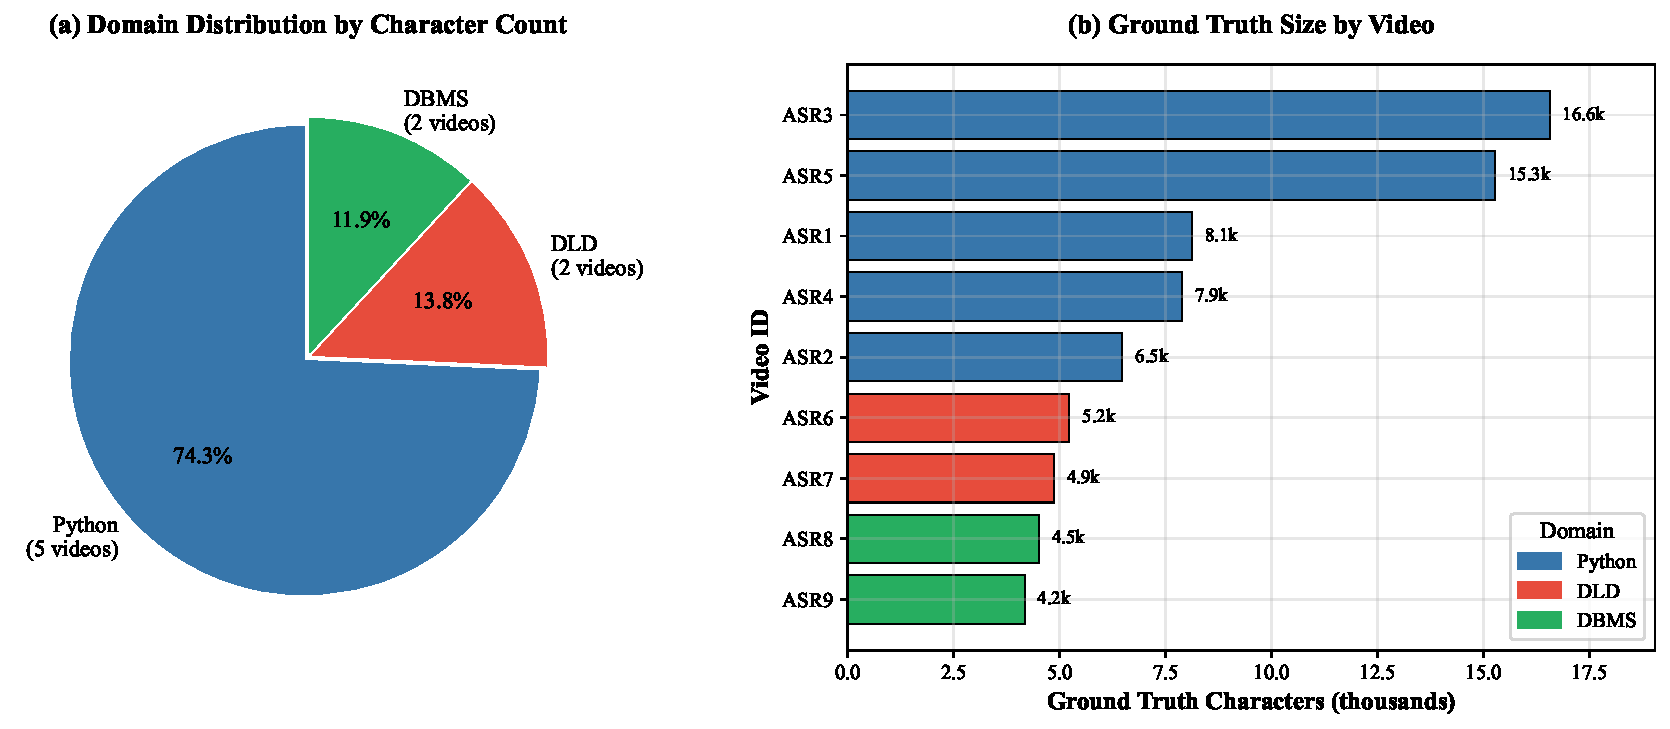
\includegraphics[width=0.95\textwidth]{figures/fig_5_7_dataset_distribution.pdf}
    \caption{Dataset Distribution: (a) Domain distribution by character count showing Python dominance with 5 videos (56\%), and DLD and DBMS each with 2 videos (22\%). (b) Ground truth size per video, ranging from 4,178 characters (BanglaASR9) to 16,558 characters (BanglaASR3).}
    \label{fig:dataset_distribution}
\end{figure}

Figure~\ref{fig:dataset_distribution} visualizes the dataset composition. The domain distribution reflects the natural availability of Banglish technical content, with Python programming lectures being most common. The character count distribution shows significant variation, with BanglaASR3 (Python Conditionals) being the longest at 16,558 characters and BanglaASR9 (SQL Queries) the shortest at 4,178 characters. This variation enables analysis of system performance across different lecture lengths.

\subsection{Ground Truth Annotation Process}

Creating accurate ground truth transcriptions required a systematic annotation process with clear guidelines and quality assurance procedures. The process involved three distinct phases.

\textbf{Phase 1: Initial Transcription.} The primary annotator listened to each recording in full, transcribing all instructor speech in Romanized Banglish. Table~\ref{tab:transcription_guidelines} summarizes the key annotation guidelines.

\begin{table}[h]
\centering
\caption{Ground Truth Transcription Guidelines}
\label{tab:transcription_guidelines}
\begin{tabular}{|l|p{5cm}|p{5.5cm}|}
\hline
\textbf{Aspect} & \textbf{Guideline} & \textbf{Example} \\
\hline
Bengali Romanization & Use common spellings; prefer simpler forms & ``amra'' not ``aamraa'' or ``amara'' \\
\hline
Technical Terms & Preserve English terms exactly as spoken & ``variable'', ``function'', ``SELECT'' \\
\hline
Code-Mixed Words & Transcribe as single unit & ``create korbo'' (will create) \\
\hline
Disfluencies & Include significant ones; omit minor fillers & Include ``umm'' pauses; omit brief ``uh'' \\
\hline
Inaudible Content & Mark explicitly & ``[inaudible]'' \\
\hline
Numbers & Use digits for technical contexts & ``variable x equals 5'' → ``variable x = 5'' \\
\hline
\end{tabular}
\end{table}

\textbf{Phase 2: Verification and Correction.} A second pass through each recording verified transcription accuracy, correcting errors identified during review. Particular attention was paid to technical terms, which are critical for our evaluation focus.

\textbf{Phase 3: Technical Review.} A domain expert familiar with the technical subject matter reviewed each transcript to verify that technical terminology was correctly transcribed and appropriately standardized.

\subsection{Keyword Annotation}

Beyond full transcription, we annotated technical keywords for term-based evaluation metrics. Keywords were identified based on the following criteria: (1) domain-specific technical terms (e.g., ``variable,'' ``loop,'' ``NAND gate''); (2) programming language keywords and built-in functions (e.g., ``print,'' ``int,'' ``SELECT''); and (3) concepts explicitly emphasized by the instructor.

Table~\ref{tab:keyword_stats} summarizes keyword statistics across the dataset.

\begin{table}[h]
\centering
\caption{Keyword Annotation Statistics by Domain}
\label{tab:keyword_stats}
\begin{tabular}{|l|c|c|c|c|}
\hline
\textbf{Domain} & \textbf{Videos} & \textbf{Total Keywords} & \textbf{Unique Keywords} & \textbf{Avg/Video} \\
\hline
Python & 5 & 250 & 87 & 50.0 \\
\hline
DLD & 2 & 67 & 34 & 33.5 \\
\hline
DBMS & 2 & 59 & 28 & 29.5 \\
\hline
\textbf{Total} & \textbf{9} & \textbf{376} & \textbf{149} & \textbf{41.8} \\
\hline
\end{tabular}
\end{table}

\begin{itemize}
    \item Identify all technical terms (e.g., ``variable,'' ``function,'' ``polymorphism'')
    \item Mark domain-specific vocabulary
    \item Note code identifiers when discussed (e.g., ``print,'' ``int,'' ``SELECT'')
    \item Record frequency of each keyword
\end{itemize}

% =============================================================================
\section{Data Preprocessing}

Raw inputs require systematic preprocessing before model processing. This section details the preprocessing pipelines for video, audio, visual, and text data, ensuring consistent, high-quality inputs for each system component.

\subsection{Video and Audio Preprocessing}

The preprocessing pipeline transforms raw video files into the audio and visual inputs required by our models. Figure~\ref{fig:preprocessing_pipeline} illustrates the complete preprocessing workflow.

% [FIGURE 5.8: Complete Preprocessing Pipeline]
% Create as a comprehensive flow diagram:
%
%    ┌─────────────────────────────────────┐
%    │     INPUT: Raw Video File (.mp4)   │
%    └───────────────┬─────────────────────┘
%                    │
%         ┌─────────┴─────────┐
%         │                   │
%         ▼                   ▼
%    ┌─────────────┐    ┌─────────────┐
%    │   AUDIO     │    │   VIDEO     │
%    │ EXTRACTION  │    │  SAMPLING   │
%    └──────┬──────┘    └──────┬──────┘
%           │                  │
%           ▼                  ▼
%    ┌─────────────┐    ┌─────────────┐
%    │  Resample   │    │   Extract   │
%    │  to 16kHz   │    │   Frames    │
%    └──────┬──────┘    └──────┬──────┘
%           │                  │
%           ▼                  ▼
%    ┌─────────────┐    ┌─────────────┐
%    │   Convert   │    │   Convert   │
%    │  to Mono    │    │  BGR→RGB    │
%    └──────┬──────┘    └──────┬──────┘
%           │                  │
%           ▼                  ▼
%    ┌─────────────┐    ┌─────────────┐
%    │  Normalize  │    │   Save as   │
%    │   Levels    │    │   JPEG 95   │
%    └──────┬──────┘    └──────┬──────┘
%           │                  │
%           ▼                  ▼
%    ┌─────────────┐    ┌─────────────┐
%    │   OUTPUT:   │    │   OUTPUT:   │
%    │  16kHz WAV  │    │ Frame JPEGs │
%    └─────────────┘    └─────────────┘
%
% Place as Figure 5.8.

\subsubsection{Audio Stream Processing}

Audio preprocessing converts the video's audio track to Whisper's expected format through a series of transformations. Table~\ref{tab:audio_preprocessing} details each step.

\begin{table}[h]
\centering
\caption{Audio Preprocessing Pipeline Steps}
\label{tab:audio_preprocessing}
\begin{tabular}{|c|l|p{4cm}|p{4.5cm}|}
\hline
\textbf{Step} & \textbf{Operation} & \textbf{Parameters} & \textbf{Purpose} \\
\hline
1 & Extract audio & FFmpeg demux & Separate audio from video container \\
\hline
2 & Resample & 16,000 Hz & Match Whisper's expected sample rate \\
\hline
3 & Channel mix & Mono (1 channel) & Reduce complexity; speech is mono \\
\hline
4 & Normalize & Peak at -1 dB & Prevent clipping; ensure adequate signal \\
\hline
5 & Encode & 16-bit PCM WAV & Uncompressed format for quality \\
\hline
\end{tabular}
\end{table}

The entire audio preprocessing pipeline is implemented as a single FFmpeg command, ensuring atomic execution and consistent output:

\begin{verbatim}
ffmpeg -i input.mp4 -ar 16000 -ac 1 -c:a pcm_s16le -af 
    "loudnorm=I=-16:TP=-1.5:LRA=11" output.wav
\end{verbatim}

This command applies resampling, mono conversion, and loudness normalization in a single pass, typically completing in under one second for a ten-minute video.

\subsubsection{Visual Stream Processing}

Frame preprocessing extracts and prepares visual samples for VLM processing. The algorithm proceeds as follows:

\begin{enumerate}
    \item \textbf{Duration Calculation:} Read video metadata to determine total duration and frame count
    \item \textbf{Timestamp Generation:} Generate sampling timestamps at configured intervals (default: 20 seconds)
    \item \textbf{Frame Extraction:} For each timestamp, seek to position and extract frame using OpenCV \cite{Bradski2000}
    \item \textbf{Color Conversion:} Convert from BGR (OpenCV default) to RGB for model compatibility
    \item \textbf{Quality Encoding:} Save as JPEG with quality setting 95 (balancing size and fidelity)
    \item \textbf{Metadata Recording:} Store timestamp association for temporal alignment
\end{enumerate}

For videos with low visual quality or challenging lighting conditions, we optionally apply image enhancement techniques: CLAHE (Contrast Limited Adaptive Histogram Equalization) for low-contrast frames with washed-out whiteboards, bilateral filtering for denoising high-noise frames from low-quality cameras, and unsharp masking for sharpening blurry frames where text edges are unclear.

\subsection{Text Preprocessing for Evaluation}

Consistent text preprocessing is essential for reliable evaluation. Both predicted transcripts and ground truth undergo identical normalization to ensure fair comparison. This normalization pipeline converts all text to NFC Unicode form, transforms to lowercase, collapses multiple whitespace characters to single spaces, removes punctuation for term matching (e.g., ``print()'' becomes ``print''), and preserves numeric digits as-is. These transformations ensure that superficial differences in formatting do not affect metric computation.

\subsection{Preprocessing Output Summary}

The preprocessing pipeline produces a standardized set of outputs for each video, organized in a consistent directory structure. Table~\ref{tab:preprocessed_outputs} summarizes all outputs.

\begin{table}[h]
\centering
\caption{Preprocessing Pipeline Outputs}
\label{tab:preprocessed_outputs}
\begin{tabular}{|l|l|p{6cm}|}
\hline
\textbf{Output} & \textbf{Format} & \textbf{Description} \\
\hline
Audio file & WAV (16kHz, mono, 16-bit) & Whisper-compatible audio \\
\hline
Frame images & JPEG (quality 95) & Sampled frames at 20s intervals \\
\hline
Frame metadata & JSON & Timestamps, frame numbers, quality flags \\
\hline
Video metadata & JSON & Duration, resolution, FPS, audio properties \\
\hline
\end{tabular}
\end{table}

% =============================================================================
\section{Implementation Details}
\label{sec:implementation_details}

This section provides comprehensive implementation details, covering the software architecture, memory management strategies essential for operating within hardware constraints, and the processing workflows that orchestrate system components.

\subsection{Software Architecture and Technology Stack}

Our implementation follows software engineering best practices, emphasizing modularity, configurability, and robustness. The system is implemented in Python 3.10, chosen for its extensive ecosystem of machine learning libraries and ease of integration with state-of-the-art models. The deep learning components are built on PyTorch \cite{Paszke2019} with the Hugging Face Transformers library \cite{Wolf2020} providing standardized interfaces to pre-trained models.

Table~\ref{tab:techstack_full} provides a comprehensive overview of the technology stack, organized by functional category.

\begin{table}[h]
\centering
\caption{Complete Technology Stack}
\label{tab:techstack_full}
\begin{tabular}{|l|l|l|p{4cm}|}
\hline
\textbf{Category} & \textbf{Library} & \textbf{Version} & \textbf{Purpose} \\
\hline
\multicolumn{4}{|c|}{\textit{Deep Learning Framework}} \\
\hline
Core & PyTorch & 2.1.0 & Tensor operations, GPU acceleration \\
\hline
Inference & Transformers & 4.37.0 & Model loading, inference pipelines \\
\hline
Quantization & BitsAndBytes & 0.41.0 & 4-bit model quantization \\
\hline
\multicolumn{4}{|c|}{\textit{Speech Processing}} \\
\hline
ASR & OpenAI Whisper & large-v3-turbo & Speech-to-text transcription \\
\hline
Audio I/O & FFmpeg & 6.0 & Audio extraction, format conversion \\
\hline
Audio Analysis & librosa & 0.10.0 & Audio quality assessment \\
\hline
\multicolumn{4}{|c|}{\textit{Visual Processing}} \\
\hline
Video I/O & OpenCV & 4.8.0 & Frame extraction, image processing \\
\hline
VLM & Qwen2.5-VL-7B & via Transformers & Visual content extraction \\
\hline
\multicolumn{4}{|c|}{\textit{Text Processing}} \\
\hline
Fuzzy Matching & RapidFuzz & 3.0.0 & String similarity computation \\
\hline
NLP & NLTK & 3.8.0 & Tokenization, text processing \\
\hline
\multicolumn{4}{|c|}{\textit{Infrastructure}} \\
\hline
Configuration & PyYAML & 6.0 & YAML configuration parsing \\
\hline
Validation & Pydantic & 2.0 & Configuration validation \\
\hline
Progress & tqdm & 4.66.0 & Progress bars for batch processing \\
\hline
\end{tabular}
\end{table}

\subsection{Memory Management Architecture}

Operating within the 24GB VRAM constraint of our target GPU (NVIDIA RTX 3090) requires careful memory management. Our three primary models---Whisper (6GB), Qwen2.5-VL (16GB), and Qwen2.5 (16GB)---cannot coexist in memory. We address this through a model registry architecture that enforces sequential loading with explicit cleanup.

% [FIGURE 5.9: GPU Memory Usage Timeline]
% Create as a timeline/Gantt chart showing VRAM usage:
%
%    PROCESSING TIMELINE
%    ═══════════════════════════════════════════════════════════════
%    
%    STAGE 1: Audio Processing (Whisper)
%    ├─────────────────────────────────────────────────────────────┤
%    │▓▓▓▓▓▓▓▓▓▓▓▓░░░░░░░░░░░░░░░░░░░░░░░░░░░░░░░░░░░░░░░░░░░░░░│
%    │ Whisper (6GB)                                               │
%    │ Peak: 8GB with processing overhead                          │
%    └─────────────────────────────────────────────────────────────┘
%                    │
%                    ▼ Unload Whisper, clear CUDA cache
%    
%    STAGE 2: Visual Processing (Qwen2.5-VL)
%    ├─────────────────────────────────────────────────────────────┤
%    │▓▓▓▓▓▓▓▓▓▓▓▓▓▓▓▓▓▓▓▓▓▓▓▓▓▓▓▓▓▓▓▓░░░░░░░░░░░░░░░░░░░░░░░░░░│
%    │ Qwen2.5-VL-7B (16GB)                                        │
%    │ Peak: 18GB with frame batching                              │
%    └─────────────────────────────────────────────────────────────┘
%                    │
%                    ▼ Unload VLM, clear CUDA cache
%    
%    STAGE 3: Content Synthesis (Qwen2.5)
%    ├─────────────────────────────────────────────────────────────┤
%    │▓▓▓▓▓▓▓▓▓▓▓▓▓▓▓▓▓▓▓▓▓▓▓▓▓▓▓▓▓▓▓▓░░░░░░░░░░░░░░░░░░░░░░░░░░│
%    │ Qwen2.5-7B-Instruct (16GB, or 6GB with 4-bit quant)         │
%    │ Peak: 18GB full precision, 8GB quantized                    │
%    └─────────────────────────────────────────────────────────────┘
%    
%    VRAM Scale: |░░░░░░░░░░░░░░░░░░░░░░░░| = 24GB
%                 0GB                    24GB
%
% Place as Figure 5.9.

Figure~\ref{fig:memory_timeline} illustrates GPU memory usage across the processing pipeline. The sequential loading strategy ensures that peak memory usage never exceeds 18GB, leaving headroom for processing overhead and operating system requirements.

The model registry implements the following memory management protocol:

\begin{enumerate}
    \item \textbf{Pre-loading Check:} Before loading a model, verify sufficient VRAM is available
    \item \textbf{Exclusive Loading:} Enforce that only one large model (VRAM $>$ 4GB) is loaded at any time
    \item \textbf{Explicit Unloading:} Delete model references and call \texttt{torch.cuda.empty\_cache()}
    \item \textbf{Garbage Collection:} Force Python garbage collection after unloading
    \item \textbf{Memory Verification:} Confirm VRAM is released before loading next model
\end{enumerate}

Table~\ref{tab:memory_stages} details the memory profile at each processing stage.

\begin{table}[h]
\centering
\caption{Memory Profile by Processing Stage}
\label{tab:memory_stages}
\begin{tabular}{|l|l|c|c|c|}
\hline
\textbf{Stage} & \textbf{Model} & \textbf{Model VRAM} & \textbf{Peak VRAM} & \textbf{Duration} \\
\hline
1. Audio Processing & Whisper large-v3-turbo & 6 GB & 8 GB & $\sim$2 min \\
\hline
2. Visual Processing & Qwen2.5-VL-7B & 16 GB & 18 GB & $\sim$5 min \\
\hline
3. Content Synthesis & Qwen2.5-7B (4-bit) & 6 GB & 8 GB & $\sim$1 min \\
\hline
\end{tabular}
\end{table}

\subsection{Processing Workflow}

The complete processing workflow for a single video involves twelve distinct steps, organized into four phases. Figure~\ref{fig:processing_workflow} provides a detailed flowchart.

% [FIGURE 5.10: Complete Video Processing Workflow]
% Create as a detailed flowchart:
%
%    ┌─────────────────────────────────────────────────────────────┐
%    │                    INPUT: Video File                        │
%    └─────────────────────────────┬───────────────────────────────┘
%                                  │
%                                  ▼
%    ┌─────────────────────────────────────────────────────────────┐
%    │  PHASE 1: INITIALIZATION                                    │
%    │  ┌─────────────────┐    ┌─────────────────┐                │
%    │  │ Load Config     │───▶│Create Output Dir│                │
%    │  └─────────────────┘    └─────────────────┘                │
%    └─────────────────────────────┬───────────────────────────────┘
%                                  │
%                                  ▼
%    ┌─────────────────────────────────────────────────────────────┐
%    │  PHASE 2: PREPROCESSING                                     │
%    │  ┌─────────────────┐    ┌─────────────────┐                │
%    │  │ Extract Audio   │    │ Sample Frames   │                │
%    │  │   (FFmpeg)      │    │   (OpenCV)      │                │
%    │  └────────┬────────┘    └────────┬────────┘                │
%    │           │                      │                          │
%    │           ▼                      ▼                          │
%    │  ┌─────────────────┐    ┌─────────────────┐                │
%    │  │  16kHz WAV      │    │ JPEG Frames     │                │
%    │  └─────────────────┘    └─────────────────┘                │
%    └─────────────────────────────┬───────────────────────────────┘
%                                  │
%                                  ▼
%    ┌─────────────────────────────────────────────────────────────┐
%    │  PHASE 3: MODEL PROCESSING (Sequential)                     │
%    │                                                             │
%    │  ┌─────────────────────────────────────────────────────┐   │
%    │  │ Step 1: Load Whisper → Transcribe → Unload          │   │
%    │  └─────────────────────────────────────────────────────┘   │
%    │                          ↓                                  │
%    │  ┌─────────────────────────────────────────────────────┐   │
%    │  │ Step 2: Load Qwen2.5-VL → Extract Visual → Unload   │   │
%    │  └─────────────────────────────────────────────────────┘   │
%    │                          ↓                                  │
%    │  ┌─────────────────────────────────────────────────────┐   │
%    │  │ Step 3: Fusion (CPU) - No model required            │   │
%    │  └─────────────────────────────────────────────────────┘   │
%    │                          ↓                                  │
%    │  ┌─────────────────────────────────────────────────────┐   │
%    │  │ Step 4: Load Qwen2.5 → Generate Notes → Unload      │   │
%    │  └─────────────────────────────────────────────────────┘   │
%    └─────────────────────────────┬───────────────────────────────┘
%                                  │
%                                  ▼
%    ┌─────────────────────────────────────────────────────────────┐
%    │  PHASE 4: OUTPUT                                            │
%    │  ┌─────────────────┐    ┌─────────────────┐                │
%    │  │ Save Outputs    │───▶│  Log Metrics    │                │
%    │  └─────────────────┘    └─────────────────┘                │
%    └─────────────────────────────┬───────────────────────────────┘
%                                  │
%                                  ▼
%    ┌─────────────────────────────────────────────────────────────┐
%    │              OUTPUT: Lecture Notes + Metrics                │
%    └─────────────────────────────────────────────────────────────┘
%
% Place as Figure 5.10.

\textbf{Phase 1: Initialization.} The workflow begins by loading configuration from YAML files and creating the output directory structure. Configuration validation using Pydantic ensures all required parameters are present and valid before processing begins.

\textbf{Phase 2: Preprocessing.} Audio extraction and frame sampling proceed in parallel where possible. Audio is extracted and converted to Whisper-compatible format; frames are sampled at configured intervals and saved with timestamp metadata.

\textbf{Phase 3: Model Processing.} This phase executes the three GPU-intensive stages sequentially, with explicit memory management between stages. Each stage follows the pattern: load model $\rightarrow$ process data $\rightarrow$ save intermediate results $\rightarrow$ unload model $\rightarrow$ clear GPU memory.

\textbf{Phase 4: Output.} Final outputs are saved to disk, including the generated lecture notes, intermediate artifacts (transcript, keywords), and evaluation metrics. Processing logs capture timing and resource usage for analysis.

\subsection{Configuration System}

System behavior is controlled through a hierarchical configuration system that separates concerns and enables reproducible experiments. The configuration is organized into four main sections: (1) \textit{ASR configuration} specifies the Whisper model variant, language setting, beam size (5), temperature (0.0 for deterministic output), and VAD filtering; (2) \textit{visual processing configuration} defines the VLM model, frame sampling interval (20 seconds), and maximum frame count (50); (3) \textit{fusion configuration} sets the similarity threshold (0.85), correction threshold (0.60), temporal alignment window (60 seconds), and maximum corrections per keyword (3); and (4) \textit{summarization configuration} specifies the LLM model, quantization level (4-bit), maximum output tokens (4096), and generation temperature (0.3). This configuration-driven approach enables systematic experimentation by varying parameters without code changes.

\subsection{Error Handling and Recovery}

Robust error handling ensures the system continues processing despite individual failures. Table~\ref{tab:error_handling} describes the error categories and recovery strategies.

\begin{table}[h]
\centering
\caption{Error Categories and Recovery Strategies}
\label{tab:error_handling}
\begin{tabular}{|l|p{4cm}|p{5.5cm}|}
\hline
\textbf{Error Category} & \textbf{Example} & \textbf{Recovery Strategy} \\
\hline
Input Error & Missing file, corrupted video & Log error, skip to next video in batch \\
\hline
Memory Error & CUDA OOM during inference & Reduce batch size, retry with smaller chunks \\
\hline
Model Error & Model loading failure & Retry with fallback model if available \\
\hline
Processing Error & Frame extraction failure & Continue with available frames; flag for review \\
\hline
Output Error & Disk full, permission denied & Save to alternative location; alert user \\
\hline
\end{tabular}
\end{table}

Checkpointing after each major stage enables recovery from interruptions. The system can resume from the last completed checkpoint, avoiding redundant reprocessing of already-completed stages.

\subsection{Evaluation Infrastructure}

The evaluation infrastructure computes metrics comparing predicted transcripts against ground truth. Our primary metrics are term-based, designed to accommodate the orthographic variability inherent to Romanized Banglish. These metrics follow standard information retrieval formulations \cite{Jurafsky2000} adapted for our fuzzy matching requirements.

\textbf{Term Recall} measures the proportion of ground truth technical terms captured in the prediction:

\begin{equation}
\text{Term Recall} = \frac{|\{t \in GT : \exists p \in Pred, \text{sim}(t,p) \geq \theta\}|}{|GT|}
\end{equation}

\textbf{Term Precision} measures the proportion of predicted terms that correspond to ground truth terms:

\begin{equation}
\text{Term Precision} = \frac{|\{p \in Pred : \exists t \in GT, \text{sim}(t,p) \geq \theta\}|}{|Pred|}
\end{equation}

\textbf{Term F1} provides the harmonic mean of precision and recall:

\begin{equation}
\text{Term F1} = 2 \times \frac{\text{Precision} \times \text{Recall}}{\text{Precision} + \text{Recall}}
\end{equation}

where $GT$ is the set of ground truth terms, $Pred$ is the set of predicted terms, $\text{sim}()$ is the normalized string similarity function, and $\theta = 0.85$ is the matching threshold.

The similarity function uses normalized Levenshtein distance, implemented efficiently using the RapidFuzz library:

\begin{equation}
\text{sim}(s_1, s_2) = 1 - \frac{\text{lev}(s_1, s_2)}{\max(|s_1|, |s_2|)}
\end{equation}

where $\text{lev}(s_1, s_2)$ is the Levenshtein edit distance between strings $s_1$ and $s_2$. The RapidFuzz library provides an efficient implementation with $O(n \cdot m)$ time complexity for strings of lengths $n$ and $m$.

% =============================================================================
\section{Experimental Design}
\label{sec:experimental_design}
% =============================================================================

This section outlines the experimental design for systematically evaluating our multimodal system. The design addresses key research questions through controlled experiments that isolate the contribution of each system component.

\subsection{Research Questions}

Our experimental evaluation is structured around five research questions that progressively examine system performance from individual components to the complete pipeline:

\begin{table}[h]
\centering
\caption{Research Questions and Corresponding Evaluation Approaches}
\label{tab:research_questions}
\begin{tabular}{|c|p{6.5cm}|p{4cm}|}
\hline
\textbf{RQ} & \textbf{Question} & \textbf{Evaluation Method} \\
\hline
RQ1 & How accurately does Whisper transcribe Banglish technical lectures, and what error patterns emerge? & Baseline ASR analysis, error categorization \\
\hline
RQ2 & Can VLM-based visual analysis reliably extract technical keywords from classroom content? & Visual extraction accuracy, coverage analysis \\
\hline
RQ3 & Does cross-modal fusion improve technical term accuracy without introducing hallucinations? & Comparative experiments, ablation study \\
\hline
RQ4 & How do different fusion thresholds affect the precision-recall trade-off? & Parameter sweep experiments \\
\hline
RQ5 & What quality of lecture notes can be achieved with the complete pipeline? & End-to-end evaluation, qualitative analysis \\
\hline
\end{tabular}
\end{table}

These research questions reflect the core challenges identified in Chapter 2: handling code-mixed ASR, leveraging visual information effectively, and balancing correction benefits against hallucination risks.

\subsection{Experimental Configurations}

To isolate the contribution of each system component, we evaluate multiple configurations representing different levels of multimodal integration. Table~\ref{tab:exp_configurations} describes each configuration tested.

\begin{table}[h]
\centering
\caption{Experimental Configurations for Comparative Evaluation}
\label{tab:exp_configurations}
\begin{tabular}{|l|c|c|c|p{4.5cm}|}
\hline
\textbf{Configuration} & \textbf{ASR} & \textbf{VLM} & \textbf{Fusion} & \textbf{Description} \\
\hline
Whisper-Only & \checkmark & & & Baseline: ASR output without modification \\
\hline
Visual-Only & & \checkmark & & Visual keyword extraction without audio \\
\hline
Verification-Only & \checkmark & \checkmark & Verify & Visual confirms ASR terms, no corrections \\
\hline
Conservative Fusion & \checkmark & \checkmark & $\theta=0.80$ & Corrections only for high-confidence matches \\
\hline
Standard Fusion & \checkmark & \checkmark & $\theta=0.60$ & Balanced threshold for correction \\
\hline
Aggressive Fusion & \checkmark & \checkmark & $\theta=0.40$ & Lower threshold, more corrections applied \\
\hline
Full Pipeline & \checkmark & \checkmark & \checkmark & Complete system with summarization \\
\hline
\end{tabular}
\end{table}

% [FIGURE 5.11: Experimental Configuration Comparison]
% Create as a comparison diagram showing:
%
%    Configuration        Components Used         Expected Behavior
%    ─────────────────────────────────────────────────────────────────
%    Whisper-Only    ──▶  [ASR]                   ──▶ Baseline accuracy
%    
%    Visual-Only     ──▶  [VLM]                   ──▶ Keyword coverage
%    
%    Verification    ──▶  [ASR]──▶[VLM]           ──▶ Confidence scoring
%                              (no modify)
%    
%    Conservative    ──▶  [ASR]──▶[VLM]──▶[Fusion] ──▶ High precision,
%                              (θ=0.80)                  lower recall
%    
%    Standard        ──▶  [ASR]──▶[VLM]──▶[Fusion] ──▶ Balanced P/R
%                              (θ=0.60)
%    
%    Aggressive      ──▶  [ASR]──▶[VLM]──▶[Fusion] ──▶ Higher recall,
%                              (θ=0.40)                  risk of errors
%
% Place as Figure 5.11.

The progression from Whisper-Only through increasingly integrated configurations allows us to measure the marginal contribution of visual information and fusion at each stage.

\subsection{Evaluation Protocol}

Each experimental configuration follows a standardized evaluation protocol to ensure fair comparison:

\begin{enumerate}
    \item \textbf{Dataset Processing:} Process all 9 BanglaASR videos using the identical preprocessing pipeline
    \item \textbf{Metric Computation:} Calculate Term Recall, Term Precision, and Term F1 against ground truth
    \item \textbf{Per-Video Analysis:} Record individual video metrics to capture domain and video-specific variations
    \item \textbf{Resource Monitoring:} Log GPU memory usage, processing time, and disk I/O for each stage
    \item \textbf{Error Analysis:} Categorize and analyze correction decisions (true positive, false positive, missed)
    \item \textbf{Output Preservation:} Save all intermediate outputs for detailed post-hoc analysis
\end{enumerate}

The fuzzy matching threshold ($\theta = 0.85$) for evaluation remains constant across all experiments, providing consistent comparison criteria.

\subsection{Statistical Considerations}

With a dataset of 9 videos, statistical power is inherently limited. We address this limitation through several methodological choices:

\begin{table}[h]
\centering
\caption{Statistical Considerations and Mitigations}
\label{tab:statistical_considerations}
\begin{tabular}{|p{3.5cm}|p{8cm}|}
\hline
\textbf{Consideration} & \textbf{Mitigation Approach} \\
\hline
Small sample size ($n=9$) & Report individual video results alongside aggregates; avoid over-relying on p-values \\
\hline
Domain imbalance (5 Python, 2 DLD, 2 DBMS) & Weight analysis by domain; report domain-stratified results \\
\hline
Video length variation & Normalize metrics appropriately; report character-weighted averages \\
\hline
Ground truth subjectivity & Use consistent transcription guidelines; report inter-annotator agreement where available \\
\hline
Multiple comparisons & Focus on pre-specified hypotheses; use effect sizes rather than significance tests \\
\hline
\end{tabular}
\end{table}

Given these constraints, our analysis emphasizes practical significance (effect sizes) over statistical significance, with qualitative error analysis complementing quantitative metrics.

\subsection{Ablation Study Design}

To understand component contributions, we conduct ablation studies removing or modifying specific system elements:

\begin{itemize}
    \item \textbf{Visual Component Ablation:} Compare Whisper-Only vs. Full Pipeline to measure visual contribution
    \item \textbf{Fusion Strategy Ablation:} Compare verification-only vs. correction-enabled fusion
    \item \textbf{Threshold Sensitivity:} Sweep correction threshold from 0.3 to 0.9 in 0.1 increments
    \item \textbf{Frame Sampling Ablation:} Vary sampling interval (10s, 20s, 30s) to assess temporal coverage trade-offs
    \item \textbf{Prompt Ablation:} Compare domain-specific vs. generic VLM prompts
\end{itemize}

Each ablation isolates a single variable while holding others constant, enabling attribution of performance differences to specific design choices.

% =============================================================================
\section{Chapter Summary}
\label{sec:chapter_summary}
% =============================================================================

This chapter presented a comprehensive methodology for the Multimodal Banglish Classroom Summarizer, addressing the unique challenges of processing code-mixed educational content. The design systematically addresses the research objectives established in Chapter 1, informed by the literature review in Chapter 2.

\subsection{Key Methodological Contributions}

The methodology contributes several innovations to the lecture summarization and code-mixed speech processing domains:

\begin{table}[h]
\centering
\caption{Summary of Methodological Contributions}
\label{tab:methodology_contributions}
\begin{tabular}{|p{3.5cm}|p{8cm}|}
\hline
\textbf{Contribution} & \textbf{Description} \\
\hline
Verification-First Fusion & Visual keywords verify and correct ASR rather than independently generating content, minimizing hallucination risk \\
\hline
Temporal Alignment Strategy & 20-second frame sampling synchronized with ASR segments enables contextually appropriate corrections \\
\hline
Confidence-Based Correction & Two-threshold system (similarity + context) controls correction aggressiveness \\
\hline
BanglaASR Benchmark Dataset & 9 real classroom recordings with 73,141 characters of manually transcribed Banglish ground truth \\
\hline
Memory-Efficient Pipeline & Sequential model loading enables 40GB+ model ensemble on 24GB consumer GPU \\
\hline
Term-Based Evaluation & Fuzzy matching metrics accommodate Romanized Banglish orthographic variation \\
\hline
\end{tabular}
\end{table}

\subsection{Design Decisions Rationale}

The methodology reflects several key design decisions, each motivated by the constraints and requirements identified in earlier chapters:

\begin{enumerate}
    \item \textbf{Pre-trained Model Leverage:} Rather than training domain-specific models (infeasible given data limitations), we leverage state-of-the-art pre-trained models (Whisper, Qwen2.5-VL, Qwen2.5) and focus engineering effort on post-processing and fusion.
    
    \item \textbf{Verification Over Generation:} Visual information verifies and corrects ASR output rather than independently generating content. This conservative approach prioritizes precision over recall, appropriate for educational applications where accuracy is paramount.
    
    \item \textbf{Consumer Hardware Target:} All design decisions respect the 24GB VRAM constraint of consumer GPUs, enabling broader deployment. Sequential model loading with explicit memory management achieves this without sacrificing model quality.
    
    \item \textbf{Domain Adaptability:} Configurable prompts and parameters enable adaptation to different technical domains (programming, digital logic, databases) without code modification.
\end{enumerate}

\subsection{Reproducibility}

To ensure reproducibility, we provide:

\begin{itemize}
    \item Complete source code with documented configuration files
    \item Pre-computed ground truth transcriptions for all 9 videos
    \item Evaluation scripts computing all reported metrics
    \item Detailed hardware and software specifications
\end{itemize}

\subsection{Transition to Results}

The following chapter presents experimental results evaluating this methodology. Chapter 5 reports quantitative performance metrics across all configurations, analyzes error patterns, and provides qualitative assessment of generated lecture notes. The experimental design outlined in Section~\ref{sec:experimental_design} structures the evaluation to address each research question systematically.

% =============================================================================
% FIGURES TO CREATE (Complete List with Specifications):
% =============================================================================
%
% Figure 5.1: Research Methodology Framework
%   Type: Flowchart
%   Content: 4 phases (Design → Development → Evaluation → Iteration)
%   Tool: Draw.io or Lucidchart
%
% Figure 5.2: High-Level System Architecture  
%   Type: Block Diagram
%   Content: Input → Preprocessing → ASR/Visual → Fusion → Summary → Output
%   Tool: Draw.io with clear component boxes
%
% Figure 5.3: Whisper ASR Processing Flow
%   Type: Vertical Flowchart
%   Content: Audio → Load Model → Transcribe → Clean → Output
%   Tool: Draw.io
%
% Figure 5.4: Frame Sampling Timeline Visualization
%   Type: Timeline Diagram
%   Content: Video timeline with frame extraction points at 0s, 20s, 40s, 60s...
%   Tool: Matplotlib or Draw.io
%
% Figure 5.5: Visual Keyword Aggregation Process
%   Type: Process Diagram
%   Content: Multiple frames → VLM extraction → Deduplication → Temporal mapping
%   Tool: Draw.io
%
% Figure 5.6: Cross-Modal Fusion Flowchart
%   Type: Decision Flowchart
%   Content: ASR term → Check visual match → Apply correction decision tree
%   Tool: Draw.io with decision diamonds
%
% Figure 5.7: Dataset Distribution
%   Type: Composite (Pie + Bar Chart)
%   Content: Domain distribution (pie), Character counts per video (bar)
%   Data: Python: 54,330 chars, DLD: 10,110 chars, DBMS: 8,701 chars
%   Tool: Matplotlib/Python
%
% Figure 5.8: Complete Preprocessing Pipeline
%   Type: Flow Diagram
%   Content: Raw video → Audio extraction → Frame sampling → Normalization → Ready
%   Tool: Draw.io
%
% Figure 5.9: GPU Memory Usage Timeline
%   Type: Line Graph
%   Content: Memory usage (GB) over processing stages
%   Data: Baseline ~2GB, Whisper ~8GB, Qwen2.5-VL ~18GB, Qwen2.5 ~18GB
%   Tool: Matplotlib/Python
%
% Figure 5.10: Complete Video Processing Workflow
%   Type: Detailed Flowchart
%   Content: 4 phases with 12 steps (see specification in text)
%   Tool: Draw.io, full page width
%
% Figure 5.11: Experimental Configuration Comparison
%   Type: Comparison Diagram
%   Content: 7 configurations showing component usage
%   Tool: Draw.io
%
% =============================================================================